\documentclass[conference]{IEEEtran}
\usepackage[top=2.5 cm, bottom=2.5 cm, left=2.0 cm, right=2.0 cm]{geometry}
\geometry{letterpaper}
\usepackage[parfill]{parskip}
\usepackage{graphicx}
\usepackage{amsmath}
\usepackage{amssymb}
\usepackage{comment}
\usepackage{epstopdf}
\usepackage{subfigure}
\usepackage{extarrows}
\usepackage{minted}
\usemintedstyle{vs}
\usepackage{kbordermatrix}

\DeclareGraphicsRule{.tif}{png}{.png}{`convert #1 `dirname #1`/`basename #1 .tif`.png}



\title{Realtime 6DOF SLAM for a Quadrotor Helicopter}

\author{\IEEEauthorblockN{Stephen Chaves}
  \and
  \IEEEauthorblockN{Schuyler Cohen}
  \and
  \IEEEauthorblockN{Patrick O'Keefe}
  \and
  \IEEEauthorblockN{Paul Ozog}}

% \IEEEauthorblockA{School of Electrical and\\Computer Engineering\\
% Georgia Institute of Technology\\
% Atlanta, Georgia 30332--0250\\
% Email: http://www.michaelshell.org/contact.html}



\begin{document}
\maketitle



\begin{abstract}
  Lorem ipsum dolor sit amet, consectetur adipisicing elit, sed do eiusmod tempor incididunt
  ut labore et dolore magna aliqua. Ut enim ad minim veniam, quis nostrud exercitation
  ullamco laboris nisi ut aliquip ex ea commodo consequat. Duis aute irure dolor in
  reprehenderit in voluptate velit esse cillum dolore eu fugiat nulla pariatur. Excepteur
  sint occaecat cupidatat non proident, sunt in culpa qui officia deserunt mollit anim id
  est laborum.
\end{abstract}






\section{Introduction}
\label{sec:introduction}

% Schuyler's section

Lorem ipsum dolor sit amet, consectetur adipisicing elit, sed do eiusmod tempor incididunt
ut labore et dolore magna aliqua. Ut enim ad minim veniam, quis nostrud exercitation
ullamco laboris nisi ut aliquip ex ea commodo consequat. Duis aute irure dolor in
reprehenderit in voluptate velit esse cillum dolore eu fugiat nulla pariatur. Excepteur
sint occaecat cupidatat non proident, sunt in culpa qui officia deserunt mollit anim id
est laborum.




\section*{System Architecture}
\label{sec:systemarchitecture}

% Steve's Section

Lorem ipsum dolor sit amet, consectetur adipisicing elit, sed do eiusmod tempor incididunt
ut labore et dolore magna aliqua. Ut enim ad minim veniam, quis nostrud exercitation
ullamco laboris nisi ut aliquip ex ea commodo consequat. Duis aute irure dolor in
reprehenderit in voluptate velit esse cillum dolore eu fugiat nulla pariatur. Excepteur
sint occaecat cupidatat non proident, sunt in culpa qui officia deserunt mollit anim id
est laborum.




\section{Incremental Smoothing and Mapping}
\label{sec:incrementalsmoothingandmapping}

%Pat's section

Incremental smoothing and mapping (iSAM) is a relatively recent approach to solving the
full SLAM problem. \cite{Kaess08tro} The full SLAM problem, in contrast to the online SLAM
problem, recovers the full posterior of the robot trajectory and landmark positions
instead of just the current robot pose and landmark positions. \cite{thrun2005probabilistic}

In standard least-squares SLAM, we solve a system of equations such as

\begin{align*}
  \Delta x' &= \underset{\Delta x}{\operatorname{argmin}} (J\Delta x - r)^{\text{T}}
\Sigma^{-1} (J\Delta x - r) \\
  &= \underset{\Delta x}{\operatorname{argmin}} \| J\Delta x - r \|^2_{\Sigma}
\end{align*}

where $J$ is the Jacobian of the system, $x$ is the state vector that contains all robot
poses and landmark positions, and $r$ is the residual of observations versus the predicted
measurements. The minimizing solution results in the standard normal equations.

\[
(J^{\text{T}} \Sigma^{-1} J) \Delta x = J^{\text{T}} \Sigma^{-1}r
\]

This is solved via the Cholesky decomposition of the information matrix,
$J^{\text{T}}\Sigma^{-1}J$.

iSAM makes a change to this problem formulation by considering the Cholesky decomposition
of $\Sigma^{-1}$ -- written as $\Sigma^{-\text{T}/2}$ to denote the upper triangular
result of the decomposition --  and rewriting the least squares problem as

\begin{align*}
    \Delta x' &= \underset{\Delta x}{\operatorname{argmin}} (J\Delta x - r)^{\text{T}}
\Sigma^{-1/2}\Sigma^{-\text{T}/2} (J\Delta x - r) \\
  &= \underset{\Delta x}{\operatorname{argmin}} \| \Sigma^{-\text{T}/2}(J\Delta x - r)
  \|^2\\
&= \underset{\Delta x}{\operatorname{argmin}} \| (A\Delta x - b)\|^2
\end{align*}

where

\begin{align*}
  A &= \Sigma^{-\text{T}/2}J \\
  b &= \Sigma^{-\text{T}/2}r
\end{align*}

This allows us to solve $A\Delta x = b$ by applying QR factorization directly to $A$. This
is advantageous because it avoids the squaring of the matrix condition number that is
associated with the normal equation form. \cite{Kaess08tro}

iSAM recovers the posterior by doing fast incremental updates to the factorization of $A$.
This means that calculations are only performed on elements that are actually affected* by
 new measurements. We can get away with this because we often have a very good estimate of
 the state vector so doing a full batch re-linearization and solution at each step wastes
 calculations because most elements of $\Delta x$ will be zero. However, iSAM periodically
 does perform a full batch solution in order to compensate for accumulated linearization
 errors. Over time, loop closures greatly decrease the sparsity of the matrix
 factorization, so variable reordering is performed during each batch solution step. The
 incremental update and variable reordering will be covered below.


\subsection*{Givens Rotations}
\label{sub:givensrotations}

The $R$ term that results from the QR decomposition of $A$ is upper triangular by
definition. When a new measurement row is added to $A$, we can incrementally update $R$
instead of performing the entire QR decomposition again. The way to achieve this is via
Givens rotations. 

Givens rotations are a way to introduce a zero at a specified point in a matrix by
premultiplying by a matrix of the form


\[
G(i, k, \theta) =
\kbordermatrix{  & & &i& &k & & \\
 & 1   & \cdots &    0   & \cdots &    0   & \cdots &    0   \\
 & \vdots & \ddots & \vdots &        & \vdots &        & \vdots \\
i & 0   & \cdots &    c   & \cdots &    -s   & \cdots &    0   \\
 & \vdots &        & \vdots & \ddots & \vdots &        & \vdots \\
k & 0   & \cdots &   s   & \cdots &    c   & \cdots &    0   \\
 & \vdots &        & \vdots &        & \vdots & \ddots & \vdots \\
 & 0   & \cdots &    0   & \cdots &    0   & \cdots &    1
       }
\] 

where $c = \cos{(\theta)}$ and $s = \sin{(\theta)}$ for some $\theta$. We follow the
  algorithms in Golub and Van Loan's \emph{Matrix Computations} to find $c$ and $s$ to
  zero a particular element in a matrix. \cite{golub1996matrix} 

When we receive new rows for $A$ when a new measurement occurs, they are appended to $R$,
which is then no longer upper-triangular. A series of Givens rotations are applied to the
elements that are below the diagonal. This is called triangularization and once the
below-diagonal elements have been removed via the rotations, the resulting
upper-triangular matrix is equivalent to the QR decomposition of the full $A$ matrix.
\cite{golub1996matrix} The same series of rotations needs to be applied to our right hand
side $b$ term.

After the rotations have been performed, the system can be solved with simple back-substitution.


\subsection*{Variable Reordering}
\label{sub:variablereordering}

Lorem ipsum dolor sit amet, consectetur adipisicing elit, sed do eiusmod tempor incididunt
ut labore et dolore magna aliqua. Ut enim ad minim veniam, quis nostrud exercitation
ullamco laboris nisi ut aliquip ex ea commodo consequat. Duis aute irure dolor in
reprehenderit in voluptate velit esse cillum dolore eu fugiat nulla pariatur. Excepteur
sint occaecat cupidatat non proident, sunt in culpa qui officia deserunt mollit anim id
est laborum.


\begin{figure}[!h]
  \begin{center}
    \subfigure[] {
    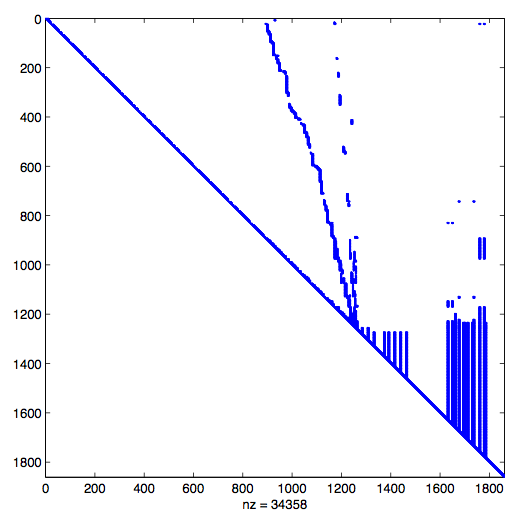
\includegraphics[width=2.5in]{images/reorder32}
    \label{fig:images/reorderResult32Resized}}
    \subfigure[] {
    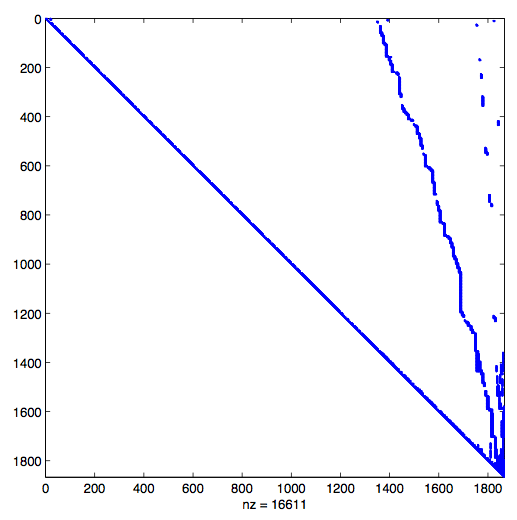
\includegraphics[width=2.5in]{images/reorder33}
    \label{fig:images/reorderResult33Resized}}
    \caption{asdfasdf}
    \label{fig:reorder}
  \end{center}
\end{figure}






\section{AprilTags}
\label{sec:apriltags}

% Paul's section

Lorem ipsum dolor sit amet, consectetur adipisicing elit, sed do eiusmod tempor incididunt
ut labore et dolore magna aliqua. Ut enim ad minim veniam, quis nostrud exercitation
ullamco laboris nisi ut aliquip ex ea commodo consequat. Duis aute irure dolor in
reprehenderit in voluptate velit esse cillum dolore eu fugiat nulla pariatur. Excepteur
sint occaecat cupidatat non proident, sunt in culpa qui officia deserunt mollit anim id
est laborum.









\section{Experiments}
\label{sec:experiments}

Lorem ipsum dolor sit amet, consectetur adipisicing elit, sed do eiusmod tempor incididunt
ut labore et dolore magna aliqua. Ut enim ad minim veniam, quis nostrud exercitation
ullamco laboris nisi ut aliquip ex ea commodo consequat. Duis aute irure dolor in
reprehenderit in voluptate velit esse cillum dolore eu fugiat nulla pariatur. Excepteur
sint occaecat cupidatat non proident, sunt in culpa qui officia deserunt mollit anim id
est laborum.


\subsection*{Simulation}
\label{sub:simulation}

% Pat's section

Lorem ipsum dolor sit amet, consectetur adipisicing elit, sed do eiusmod tempor incididunt
ut labore et dolore magna aliqua. Ut enim ad minim veniam, quis nostrud exercitation
ullamco laboris nisi ut aliquip ex ea commodo consequat. Duis aute irure dolor in
reprehenderit in voluptate velit esse cillum dolore eu fugiat nulla pariatur. Excepteur
sint occaecat cupidatat non proident, sunt in culpa qui officia deserunt mollit anim id
est laborum.

\begin{figure}[!t]
  \centering
  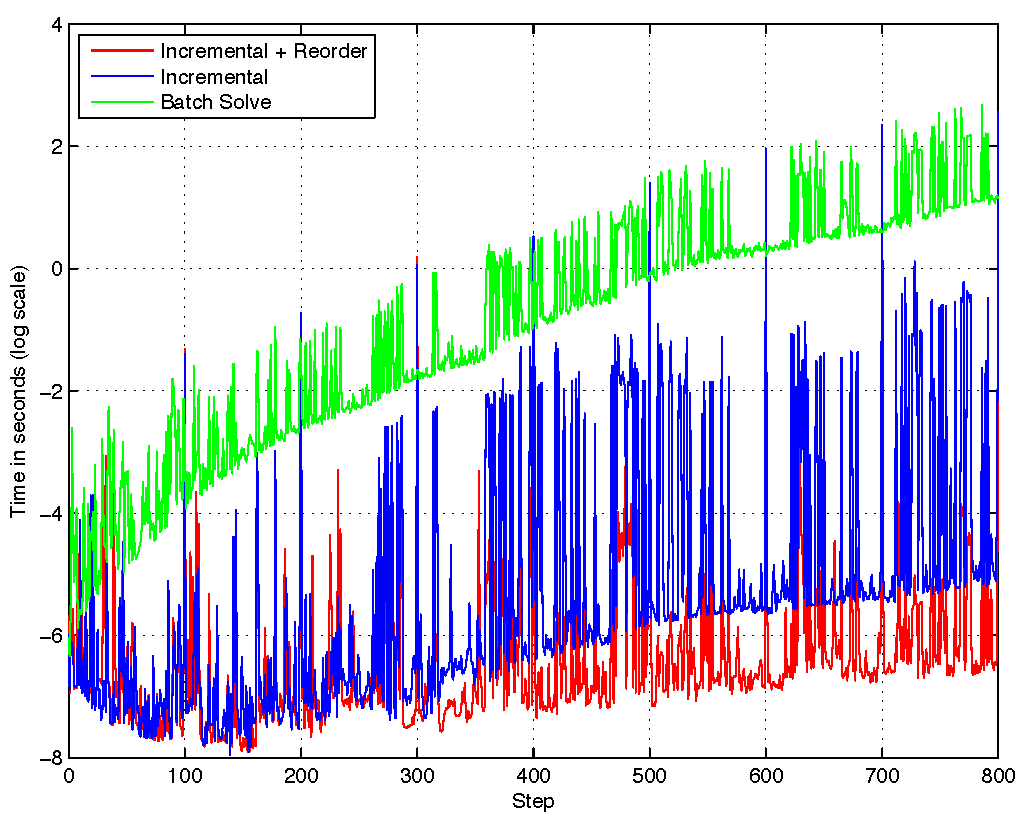
\includegraphics[width=2.5in]{images/stepTimeResults}
  \caption{The time per step for different SLAM solve methods.}
  \label{fig:stepTime}
\end{figure}


\subsection*{Parrot AR.Drone}
\label{sub:quadrotor}

% Steve talks about drone hardware
% Schuyler gets results

Lorem ipsum dolor sit amet, consectetur adipisicing elit, sed do eiusmod tempor incididunt
ut labore et dolore magna aliqua. Ut enim ad minim veniam, quis nostrud exercitation
ullamco laboris nisi ut aliquip ex ea commodo consequat. Duis aute irure dolor in
reprehenderit in voluptate velit esse cillum dolore eu fugiat nulla pariatur. Excepteur
sint occaecat cupidatat non proident, sunt in culpa qui officia deserunt mollit anim id
est laborum.










\section{Conclusion}
\label{sec:conclusion}

% Schuyler's section

Lorem ipsum dolor sit amet, consectetur adipisicing elit, sed do eiusmod tempor incididunt
ut labore et dolore magna aliqua. Ut enim ad minim veniam, quis nostrud exercitation
ullamco laboris nisi ut aliquip ex ea commodo consequat. Duis aute irure dolor in
reprehenderit in voluptate velit esse cillum dolore eu fugiat nulla pariatur. Excepteur
sint occaecat cupidatat non proident, sunt in culpa qui officia deserunt mollit anim id
est laborum.



\section*{Acknowledgment}

The authors would like to thank Sprite, the number 7, and Emacs.



\bibliographystyle{IEEEtran}
% argument is your BibTeX string definitions and bibliography database(s)
\bibliography{IEEEabrv,references}


\end{document}



% An example of a floating table. Note that, for IEEE style tables, the
% \caption command should come BEFORE the table. Table text will default to
% \footnotesize as IEEE normally uses this smaller font for tables.
% The \label must come after \caption as always.
%
% \begin{table}[!t]
%%   increase table row spacing, adjust to taste
%   \renewcommand{\arraystretch}{1.3}
%   if using array.sty, it might be a good idea to tweak the value of
%   \extrarowheight as needed to properly center the text within the cells
%   \caption{An Example of a Table}
%   \label{table_example}
%   \centering
%%   Some packages, such as MDW tools, offer better commands for making tables
%%   than the plain LaTeX2e tabular which is used here.
%   \begin{tabular}{|c||c|}
%     \hline
%     One & Two\\
%     \hline
%     Three & Four\\
%     \hline
%   \end{tabular}
% \end{table}
